\chapter{Software}

Die Software des Systems setzt sich aus zwei Hauptkomponenten zusammen. Zur Verarbeitung der eingehenden CAN-Nachrichten wird eine ESP32 verwendet, der auf dem espidf-Framework basiert. Dieser Microcontroller übernimmt nicht nur das Empfangen der Nachrichten, sondern zeigt diese auch auf einem LCD-Display an und stellt sie über eine REST-API zur Verfügung. Um eine benutzerfreundlichere Oberfläche zu bieten, wurde zusätzlich eine GUI entwickelt. Diese basiert auf dem von Google entwickelten Framework Flutter. Dank dieser GUI können die CAN-Nachrichten komfortabel über eine Windows-Anwendung, einen Browser oder einer App ausgelesen werden. Das Architekturbild \ref{fig:architekturbild} stellt die grundsätzliche Architektur des Systems dar. Auf die einzelnen Komponenten wird im folgendem genauer eingegangen.
\begin{figure}[h]
  \centering
  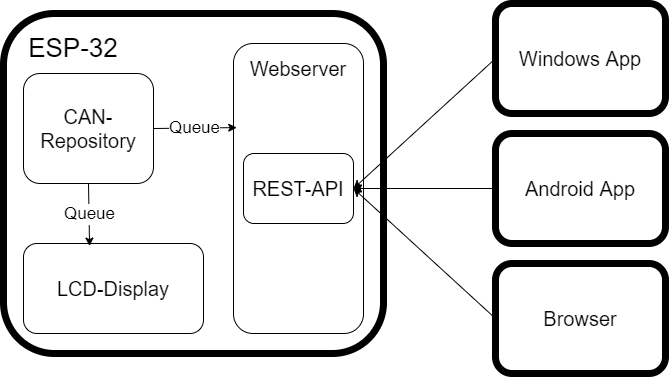
\includegraphics[width=0.8\textwidth]{img/architekturbild.drawio.png}
  \caption{Architekturbild}
  \label{fig:architekturbild}
\end{figure}


\section{ESP32}
\subsection{Architektur}
\subsubsection{Projektstruktur}
Bei der Projektstruktur \ref{fig:projektstruktur_esp} wurde sich an der Clean Architecture von Robert C. Martin orientiert \cite{martin_clean_2018}. Da diese für Objekt Orientierte Programmiersprachen ausgelegt ist, wurde die Struktur an unsere Bedürfnisse angepasst. Der Benefit der Projektstruktur ist, dass die Business Logiken, welche in den Controllern implementiert sind, von der Verarbeitung der Daten gekapselt werden. Jeder Controller ist ein FreeRTOS Task, welche die gleiche Grundstruktur, eine FSM, besitzt. Auf die FSM wird in \ref{chap:fsm} genauer eingegangen.
\begin{lstlisting}
    while (1)
    {
        switch (fsm_controller_current_state)
        {
        case STARTING:
            break;
        case CONFIGURATION:
            break;
        case OPERATION:
            break;
        }
        vTaskDelay(10);
    }
\end{lstlisting}
Der Bereich \textit{data} ist für die Verarbeitung der Daten zuständig. Hier werden die Rohdaten in geeignete Strukturen transformiert, die für die Controller leicht zu verarbeiten sind. Die Strukturen sind in \textit{models} definiert.
\begin{figure}[h]
  \centering
  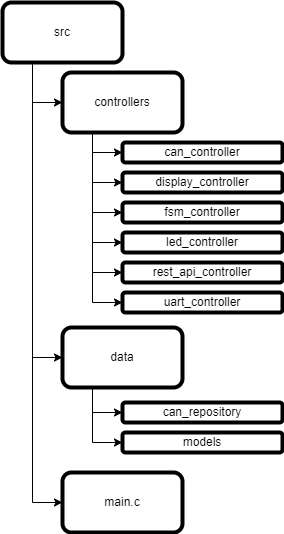
\includegraphics[height=0.7\textwidth]{img/projektstruktur.png}
  \caption{Projektstruktur ESP}
  \label{fig:projektstruktur_esp}
\end{figure}

\subsubsection{Finite State Machine}
\label{chap:fsm}
Um das Verhalten des Systems klar und strukturiert zu unterteilen, wurde eine Final State Machine (FSM) eingesetzt. Diese besteht aus den drei States \textit{STARTING}, \textit{CONFIGURATION} und \textit{OPERATION} \ref{fig:fsm}.
\begin{figure}
  \centering
  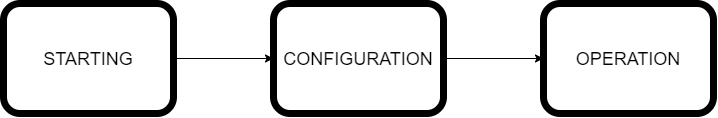
\includegraphics[width=0.8\textwidth]{img/fsm.drawio.png}
  \caption{FSM}
  \label{fig:fsm}
\end{figure}
Der State \textit{STARTING} \ref{fig:state_starting} ist für den Systemstart verantwortlich. Hierbei werden die einzelnen Controller als FreeRTOS Tasks gestartet.
\begin{figure}
  \centering
  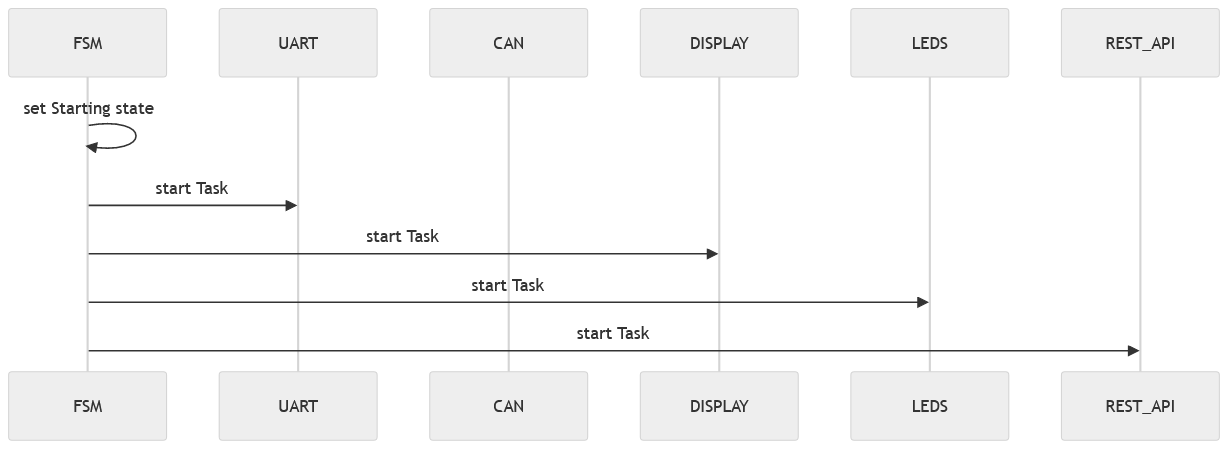
\includegraphics[width=0.8\textwidth]{img/state_starting.PNG}
  \caption{State STARTING}
  \label{fig:state_starting}
\end{figure}
Daraufhin wird in den \textit{CONFIGURATION} \ref{fig:state_configuration} State übergegangen. Hier wird das System mit den nötigen Einstellungen konfiguriert. So wird unter anderem die Baudrate des CAN Netzwerks vom User gesetzt und an den CAN Controller übertragen.
\begin{figure}
  \centering
  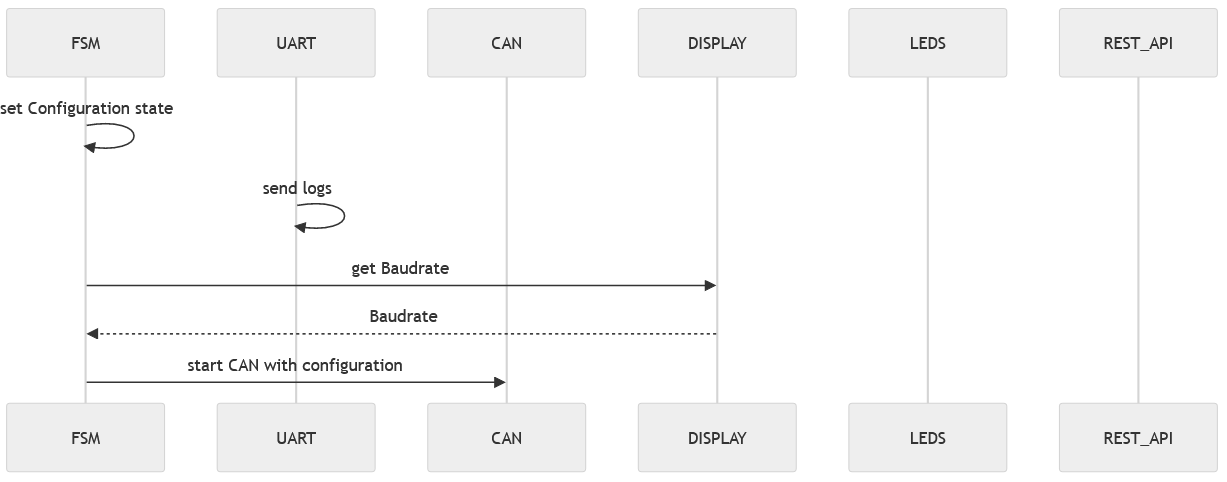
\includegraphics[width=0.8\textwidth]{img/state_configuration.PNG}
  \caption{State CONFIGURATION}
  \label{fig:state_configuration}
\end{figure}
Wenn alle Konfigurationen abgeschlossen sind, kann in den \textit{OPERATION} \ref{fig:state_operation} State gewechselt werden. In diesem Zustand wird das CAN Netzwerk laufend auf Funktionalität geprüft. Außerdem wird auf ankommende CAN Nachrichten gelauscht. Das Resultat der Funktionalitätsprüfung wird anschließend dem LED Controller mitgeteilt, sodass dieser die richtigen LEDs schalten kann. Wenn eine CAN Nachricht angekommen ist, wird diese vom CAN Repository verarbeitet und auf die jeweiligen Queues aufgeteilt. Anschließend steht die Nachricht dem LED Controller, dem Display Controller und dem REST API Controller zur Verfügung. Jetzt können von den Controllern die richtigen LEDs geschalten, sowie das Display und die REST API mit der neuen Nachricht aktualisiert werden.
\begin{figure}
  \centering
  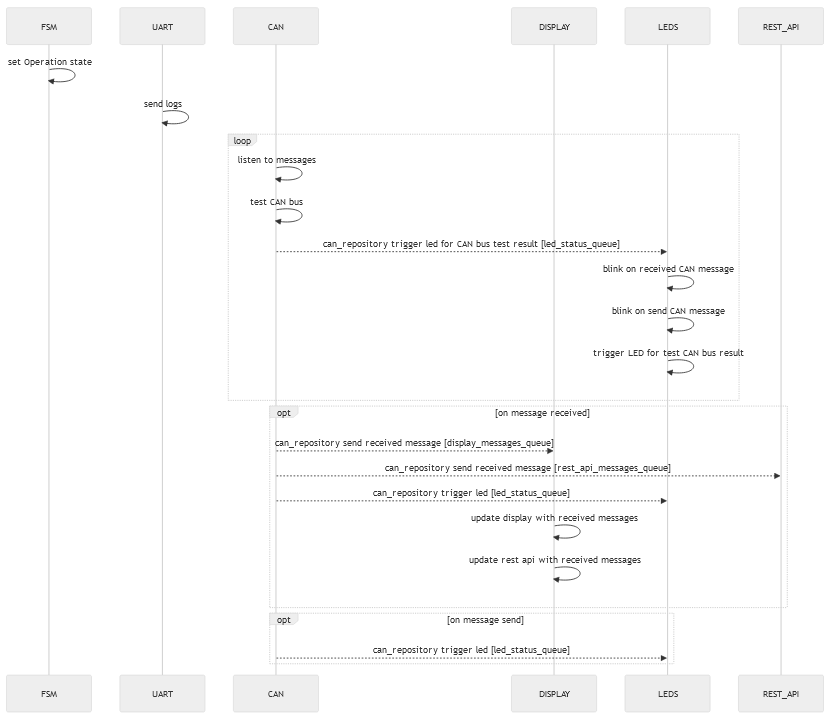
\includegraphics[width=0.8\textwidth]{img/state_operation.PNG}
  \caption{State OPERATION}
  \label{fig:state_operation}
\end{figure}

\subsection{Wichtige Komponenten}
\subsubsection{CAN Repository}
Ein zentraler Baustein der Software ist das CAN Repository mit den definierten Datenmodellen. Laut Robert C. Martins Clean Architecture \cite{martin_robert_c_clean_2012} sollten für eine saubere Software Architektur Interface Adapter implementiert werden. Die Interface Adapter sind für die Konvertierung der Daten zwischen Data Source, in unserem Fall dem CAN Controller, und den UseCases, bei uns LEDs, Display und REST API, zuständig. Durch die vorhergehende Datenkonvertierung können sich die UseCases ihrer einzigen Aufgabe, nämlich die Anzeige der Daten widmen. Mit dieser Implementierung ist auch das Single Responsibility Principle der SOLID Prinzipien erfüllt \cite{martin_robert_c_solid_2020}. Dementsprechend wurde für jeden Controller (LED, DISPLAY und REST\_API) ein entsprechendes Datenmodell definiert. Diese Datenmodelle enthalten außschließlich Informationen, die für die Anzeige der Daten mit dem jeweiligen Controller nötig sind.
\begin{lstlisting}
    #LED
    struct Led
    {
        enum Leds gpio;
        enum LedValue value;
    };
    
    #DISPLAY
    struct MessageItem
    {
        int id;
        char text[21];
    };
    
    #REST_API
    struct CanMessage
    {
        int64_t micros;
        twai_message_t message;
    };
\end{lstlisting}
Für die Konvertierung der Rohdaten des CAN Controllers, in die jeweiligen Datenmodelle wurde im CAN Repository, je eine Funktion implementiert. Danach wird das konvertierte Datenmodell in die jeweilige Queue geschrieben.
\begin{lstlisting}
static struct MessageItem twai_message_to_display_message_item(twai_message_t twai_message)
{
    struct MessageItem message_item;

    message_item.id = twai_message.identifier;

    const int index_data_start = 9;
    sprintf(message_item.text, "0x%lX", twai_message.identifier);
    const int needed_whitespaces = index_data_start - strlen(message_item.text);

    for (int i = 0; i < needed_whitespaces; i++)
    {
        strcat(message_item.text, " ");
    }

    int arrayLength = sizeof(twai_message.data) / sizeof(twai_message.data[0]);

    for (int i = 0; i < arrayLength; i++)
    {
        char item[10];
        snprintf(item, sizeof(item), "%d", twai_message.data[i]);
        strcat(message_item.text, item);
    }

    return message_item;
}

static struct CanMessage twai_message_to_can_message(twai_message_t twai_message)
{
    struct CanMessage can_message;

    int64_t uptime_micros = esp_timer_get_time();
    can_message.micros = uptime_micros;
    can_message.message = twai_message;

    return can_message;
}

extern void can_repository_distribute_received_message(twai_message_t received_twai_message)
{
    struct MessageItem received_message_item = twai_message_to_display_message_item(received_twai_message);
    xQueueSend(display_messages_queue, &received_message_item, 1);

    struct CanMessage received_can_message = twai_message_to_can_message(received_twai_message);
    xQueueSend(rest_api_messages_queue, &received_can_message, 1);

    struct Led led_blue_receive = {LED_BLUE_RECEIVE, LED_ON};
    xQueueSend(led_status_queue, &led_blue_receive, 1);
}
\end{lstlisting}
Durch diese Implementierung unter Beachtung der Clean Architecture und SOLID Prinzipien ist die Data Source von den UseCases gekapselt. Somit ist eine leichte Wartbarkeit und Erweiterbarkeit der Software gewährleistet.

\subsubsection{Display}
Das Display verfügt aktuell über zwei verschiedene Anzeigemöglichkeiten. Zum einen kann ein Menü mit beliebigen Menüeinträgen erstellt werden, zum anderen können die aktuellen CAN Messages angezeigt werden. \\
Um die Software bei Bedarf mit weiteren Menüs einfach erweitern zu können wurde das \textit{menu\_presentation} Modul so gestaltet das ein beliebiges Menü erstellt werden kann. So kann ein Array bestehend aus \textit{MenuItem} Elementen und eine Funktion \textit{void (*func\_enter)(int)} übergeben werden, welche bei betätigen des \textit{ENTER} Buttons ausgeführt wird.
\begin{lstlisting}
struct MenuItem
{
    u_int8_t id;
    u_int8_t is_selected;
    char text[50];
    void *value;
};
\end{lstlisting}
\begin{lstlisting}
extern void menu_presentation_show(i2c_lcd1602_info_t *lcd_info, struct MenuItem menu[], int menu_size, void (*func_enter)(int), enum Button button_pressed, int initial_show)
{
    char selected_string[52] = "> ";

    if (button_pressed >= 0 || initial_show)
    {
        handle_button_pressed(button_pressed, menu, menu_size, func_enter);

        i2c_lcd1602_reset(lcd_info);
        for (int i = 0; i < menu_size; i++)
        {
            i2c_lcd1602_move_cursor(lcd_info, 0, i);

            if (menu[i].is_selected)
            {
                strcat(selected_string, menu[i].text);
                i2c_lcd1602_write_string(lcd_info, selected_string);
            }
            else
            {
                i2c_lcd1602_write_string(lcd_info, menu[i].text);
            }
        }
    }
}
\end{lstlisting}
In der aktuellen Implementierung ist ein Menü zur Auswahl der Baudrate implementiert.
\begin{lstlisting}
menu_presentation_show(lcd_info, baudrate_menu, baudrate_menu_size, baudrate_menu_send_baudrate, button_pressed, false);
\end{lstlisting}
Für die Anzeige der CAN Nachrichten auf dem Display wurde ein Algorithmus entwickelt, der sicherstellt, dass sich das Display nur aktualisiert wenn nötig \ref{fig:display_controller_show_messages}. Mit dieser Implementierung wird ein Flackern des Displays vermieden. Ereignisse, die ein neuladen des Displays auslösen sind, der Empfang einer neuen CAN ID oder eine Änderung des Data Segments einer bereits enthaltenen CAN ID. Außerdem ist es möglich mit den Buttons nach oben und unten zu scrollen, um mehr als vier CAN IDs auf dem vier zeiligen Display anzeigen zu können. Auch hier wird das Display aktualisiert.
\begin{figure}
  \centering
  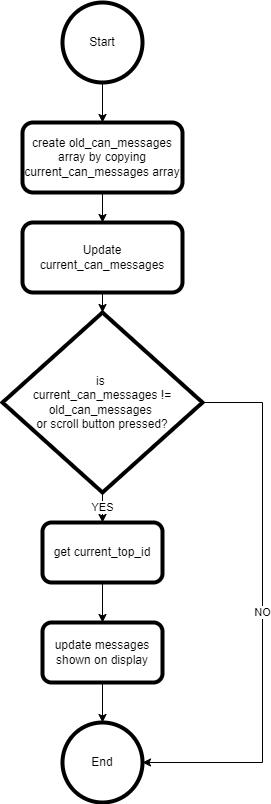
\includegraphics[height=0.8\textwidth]{img/display_controller_show_messages.png}
  \caption{Algorithmus um CAN Messages anzuzeigen}
  \label{fig:display_controller_show_messages}
\end{figure}
\subsubsection{REST API}
Um die aktuellen Nachrichten von extern leicht abfragen zu können wurde eine REST API zur Verfügung gestellt. Um auf die REST API zuzugreifen, öffnet der ESP32 den WLAN Access Point \textit{CAN-TO-GO}. Außerdem wird ein Webserver gestartet. Der Webserver stellt die Uri \textit{/can} zur Verfügung, auf welche über \textit{http://192.168.4.1/can} zugegriffen werden kann.
\begin{lstlisting}
    static httpd_uri_t get_can = {
        .uri = "/can",
        .method = HTTP_GET,
        .handler = can_get_handler,
        .user_ctx = NULL};
\end{lstlisting}
Auf dieser Seite werden die aktuellesten 100 CAN Nachrichten im JSON Format zur Verfügung gestellt.
\begin{lstlisting}
    {"messages" : [{"micros": 223754230, "id": 291, "ext": 0, "dlc": 8, "data": [0,0,1,1,0,0,0,0]},{"micros": 223864208, "id": 2047, "ext": 0, "dlc": 8, "data": [0,0,1,1,0,0,0,0]},{"micros": 223964351, "id": 35, "ext": 0, "dlc": 8, "data": [0,0,1,1,0,0,0,0]},...]}
\end{lstlisting}

\section{User Interface}
Da das Display für den Nutzer nur eine geringe Größe und eine eingeschränkte Funktionalität bietet, wurde ein externes User Interface entwickelt. Um mit einer Code Base das User Interface auf einer Vielzahl von Geräten bereitstellen zu können wurde als Framework \textit{Flutter} gewählt. Flutter ist ein Open-Source-Framework von Google, dass es erlaubt mit nur einer Code Basis das Projekt als Windows Applikation, als Web Applikation und als App auf mobilen Endgeräten zu compilieren. Als Programmiersprache wird \textit{Dart} eingesetzt.

\subsection{Funktionalitäten}
\begin{figure}[h]
  \centering
  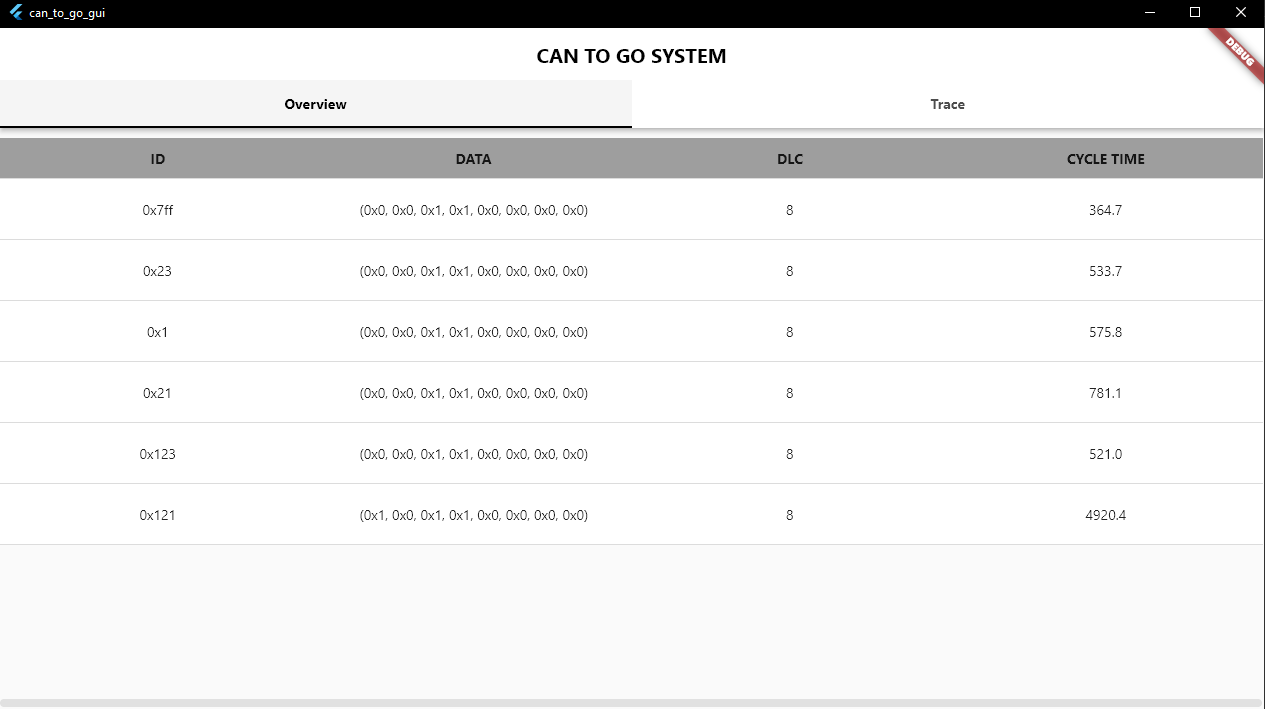
\includegraphics[width=0.9\textwidth]{img/gui_overview.PNG}
  \caption{Overview Tab}
  \label{fig:gui_overview}
\end{figure}
\begin{figure}[ht]
  \centering
  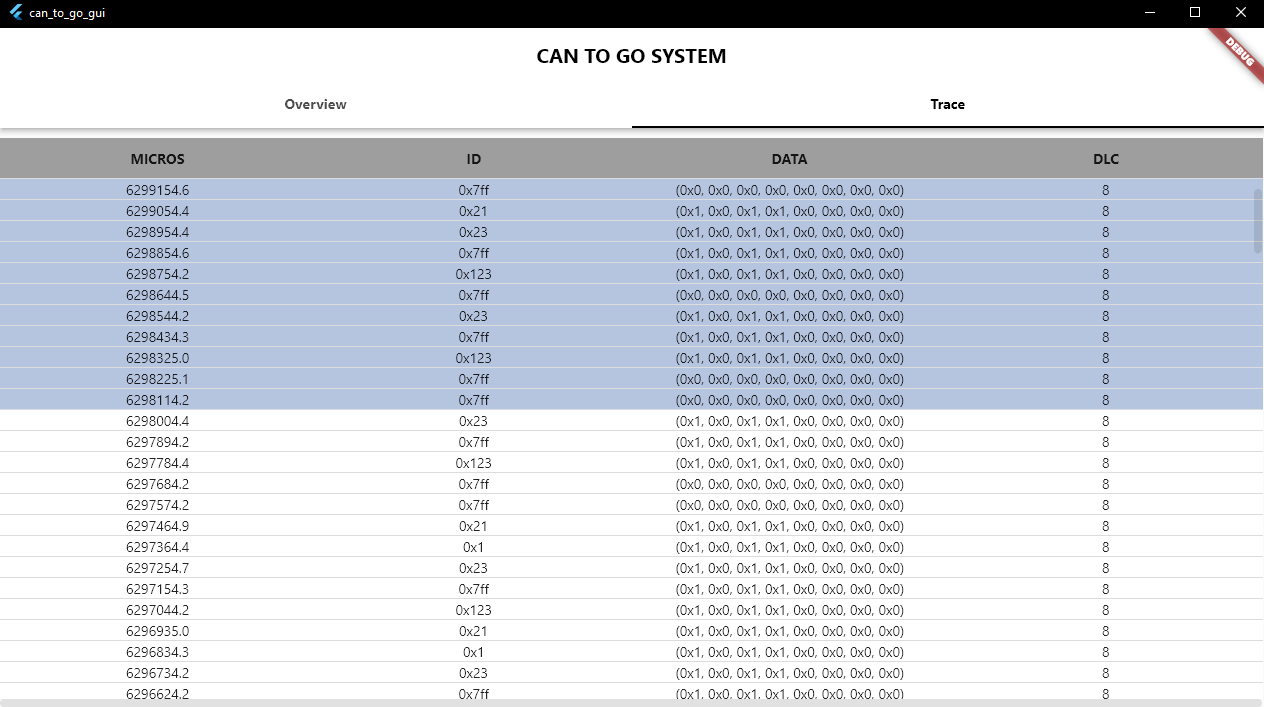
\includegraphics[width=0.9\textwidth]{img/gui_trace.PNG}
  \caption{Trace Tab}
  \label{fig:gui_trace}
\end{figure}
Das User Interface besitzt zwei verschiedene Anzeigen für den User. Zum einen gibt es ein \textit{Overview} Tab \ref{fig:gui_overview}, welches alle CAN IDs anzeigt, die empfangen wurden. Das Data Segment repräsentiert dabei immer den aktuellen Stand der jeweiligen ID. Die Cycle Time gibt darüber Auskunft, in welchem Zyklus die jeweilige CAN ID empfangen wird. \\
Außerdem gibt es die Möglichkeit über den \textit{Trace} Tab \ref{fig:gui_trace}, die letzten angekommen CAN Nachrichten zu sehen. Dabei werden die Nachrichten, die mit dem letzten Batch neu hinzugefügt wurden in einer anderen Farbe markiert, um für den User eine bessere Übersicht zu gewährleisten.

\subsection{Projektstruktur}
Bei der Projektstruktur für die GUI \ref{fig:projektstruktur_gui} wurde sich ebenfalls an der Clean Architecture von Robert C. Martin orientiert \cite{martin_clean_2018}.
Über die \textit{datasources} werden die Rohdaten von der bereitgestellten REST API gelesen und als eine Liste von \textit{CanMessageModel} zurückgegeben.
\begin{lstlisting}
    class EspRestApiRemoteDataSource {
        final String _url = "http://192.168.4.1/can";
      
        Future<List<CanMessageModel>> getCanMessages() async {
          final http.Response response = await http.get(Uri.parse(_url));
      
          List<dynamic> canMessagesJson = json.decode(response.body)["messages"];
      
          return canMessagesJson
              .map((messageJson) => CanMessageModel.fromJson(messageJson))
              .toList();
        }
      }      
\end{lstlisting}
Die Repositories sind dafür zuständig die Rohdaten in die Liste des jeweiligen Tabs zu transformieren. \\
Das \textit{CanOverviewRepository} erstellt eine Liste mit den empfangenen CAN IDs zu berechnet die Cylce Time.
\begin{lstlisting}
    Future<List<CanMessageModel>> getCanOverviewModels(bool refresh) async {
        if (refresh) {
          canMessagesCache = [];
          canMessagesUniqueIdCache = [];
        }
        final currentCanModelsBatch =
            (await espRestApiRemoteDataSource.getCanMessages()).reversed;
    
        for (CanMessageModel canMessage in currentCanModelsBatch) {
          if (!canMessagesCache.contains(canMessage)) {
            canMessagesCache.insert(0, canMessage);
          }
          if (canMessagesCache.length == 1001) {
            canMessagesCache.removeLast();
          }
        }
    
        List<CanMessageModel> currentUniqueMessages = [];
        for (CanMessageModel canMessage in canMessagesCache) {
          bool doesMessageWithIdExistInList =
              currentUniqueMessages.any((model) => model.id == canMessage.id);
          if (!doesMessageWithIdExistInList) {
            currentUniqueMessages.add(canMessage);
          }
        }
    
        for (CanMessageModel canMessage in currentUniqueMessages) {
          int index = canMessagesUniqueIdCache
              .indexWhere((item) => item.id == canMessage.id);
    
          if (canMessage.micros != 0) {
            if (index != -1) {
              canMessage.cycleTime =
                  getCycleTimeForId(canMessage.id, canMessagesCache.toList());
              canMessagesUniqueIdCache[index] = canMessage;
            } else {
              canMessagesUniqueIdCache.add(canMessage);
            }
          }
        }
    
        return canMessagesUniqueIdCache;
      }       
\end{lstlisting}
Das \textit{CanTraceRepository} erstellt eine Liste mit den letzten 200 empfangen Nachrichten und gibt zurück wie viele Nachrichten neu hinzugefügt wurden.
\begin{lstlisting}
    Future<CanTraceResult> getCanTraceModels(bool refresh) async {
        if (refresh) {
          canMessagesTrace = [];
        }
    
        final currentCanModelsBatch =
            await espRestApiRemoteDataSource.getCanMessages();
    
        int addedCount = 0;
    
        for (CanMessageModel canMessage in currentCanModelsBatch) {
          if (!canMessagesTrace.contains(canMessage)) {
            canMessagesTrace.insert(0, canMessage);
            addedCount++;
          }
          if (canMessagesTrace.length == 201) {
            canMessagesTrace.removeLast();
          }
        }
    
        return CanTraceResult(canMessagesTrace, addedCount);
      }    
\end{lstlisting}
Im \textit{presentation} Layer werden die \textit{pages} und die \textit{widgets} erstellt, die auf den jeweiligen \textit{pages} angezeigt werden. Da sowohl der \textit{Overview} Tab als auch der \textit{Trace} Tab aus einer Tabelle von CAN Nachrichten bestehen, wurde ein Widget \textit{CanTable} definiert, welches über Parameter auf das jeweilige Tab angepasst werden kann.
\begin{lstlisting}
    class CanTable extends StatelessWidget {
        final List<String> headers;
        final List<CanMessageModel> canMessages;
        final bool isOverviewTab;
        final double rowHeight;
        final int? addedCount;
    ...
    }      
\end{lstlisting}
Im \textit{Overview} Tab und im \textit{Trace} Tab wird die zuvor definierte Tabelle dann über den \textit{BuildContext} erstellt.
\begin{lstlisting}
    # Overview Tab
    Widget build(BuildContext context) {
        final List<String> headers = [
          "ID",
          "DATA",
          "DLC",
          "CYCLE TIME",
        ];
    
        return CanTable(
          headers: headers,
          rowHeight: 60.0,
          isOverviewTab: true,
          canMessages: canMessagesUniqueId,
        );
      }     
\end{lstlisting}
\begin{lstlisting}
    # Trace Tab
    Widget build(BuildContext context) {
        final List<String> headers = [
          "MICROS",
          "ID",
          "DATA",
          "DLC",
        ];
    
        return CanTable(
          headers: headers,
          rowHeight: 20.0,
          isOverviewTab: false,
          canMessages: canMessages,
          addedCount: addedCount,
        );
      }       
\end{lstlisting}

\begin{figure}
  \centering
  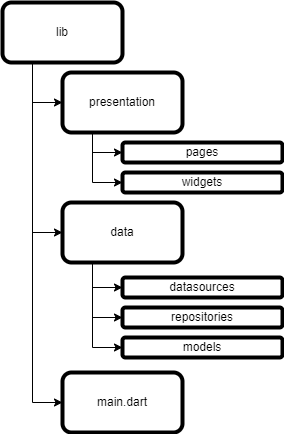
\includegraphics[height=0.7\textwidth]{img/projektstruktur_gui.png}
  \caption{Projektstruktur GUI}
  \label{fig:projektstruktur_gui}
\end{figure}